\documentclass{article}
\usepackage[utf8]{inputenc}
\usepackage{tikz, url, hyperref}
\usepackage{amsmath, amssymb, amsthm}

\tikzset{every picture/.style={line width=0.75pt}} %set default line width to 0.75pt        

\newcommand{\A}{\mathcal{A}}
\newcommand{\X}{\mathcal{X}}
\newcommand{\U}{\mathcal{U}}
\newcommand{\G}{\mathcal{G}}
\newcommand{\R}{\mathbb{R}}
\newcommand{\set}[1]{\ensuremath{\{ #1 \}}}

\theoremstyle{definition}
\newtheorem{question}{Possible research question}

%\theoremstyle{definition}
%\newtheorem{dfn}{Definition}
%\newtheorem{eg}{Example}

\title{Max-Sum and other things}
\author{Abhimanyu Pallavi Sudhir}
\date{November 2021}

\begin{document}

\maketitle

\section{Max-sum algorithm}

\subsection{Definitions and intuition}

The setting of the max-sum algorithm is a bipartite graph between choices $x_i$'s and utility function $U_j$'s (e.g. Fig~\ref{fig:bipartite}). Each $x_i$ takes values in a discrete set $X_i$, and each $U$ is a function on $\prod_{i}{X_i}$:

\begin{figure}
    \centering
    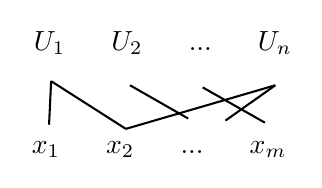
\begin{tikzpicture}[x=0.75pt,y=0.75pt,yscale=-1,xscale=1]
%uncomment if require: \path (0,235); %set diagram left start at 0, and has height of 235

%Straight Lines [id:da4743496553655544] 
\draw    (221.8,103.66) -- (220.8,124.66) ;
%Straight Lines [id:da9445033092006934] 
\draw    (221.8,103.66) -- (257.8,126.66) ;
%Straight Lines [id:da2794103208338452] 
\draw    (259.8,105.66) -- (287.8,121.66) ;
%Straight Lines [id:da45538659208567567] 
\draw    (329.8,105.66) -- (257.8,126.66) ;
%Straight Lines [id:da20672394462920862] 
\draw    (329.8,105.66) -- (305.8,122.66) ;
%Straight Lines [id:da6051041254436016] 
\draw    (294.8,106.66) -- (324.8,123.66) ;

% Text Node
\draw (212,78.4) node [anchor=north west][inner sep=0.75pt]    {$U_{1} \ \ \ \ \ U_{2} \ \ \ \ \ ...\ \ \ \ \ U_{n}$};
% Text Node
\draw (211,131.4) node [anchor=north west][inner sep=0.75pt]    {$x_{1} \ \ \ \ \ x_{2} \ \ \ \ \ ...\ \ \ \ \ x_{m}$};


\end{tikzpicture}

    \label{fig:bipartite}
\end{figure}

Each iteration, a ``message is passed from each $U_j$ to each of its neighbours $X_i$'', that is a function is calculated, $r_{ji}:X_i\to\R$ defined as:

\begin{equation}
    r_{ji}(x_i)=
    \max_{x_{-i}}\left[{U_j(x_i,x_{-i}) + \sum_{i'\ne i}{q_{i'j}(x_{i'})}}\right]
    \label{eq:utox}
\end{equation}

And a ``message is passed from each $X_i$ to each of its neighbours $U_j$'', that is a function is calculated, $q_{ij}:X_i\to\R$ defined as:

\begin{equation}
    q_{ij}(x_i) = \sum_{j'\ne j}{r_{j'i}(x_i)}
    \label{eq:xtout}
\end{equation}

Each $x_i^*$ is set to maximize $\sum_{j}{r_{ji}(x_i)}$.

When the graph is cycle-free, this algorithm \emph{globally} maximizes the ``aggregate utility'' $\sum_j{U_j}(x^*)$ \cite{rogers}.

\subsection{Link to markets}

Eq~\ref{eq:utox} essentially allows each agent $i$ whose actions affect stakeholder $j$ to take into account the demand from stakeholder $j$, $U_j(x_i,x_{-i})$, and the derived demand from $i'$, $q_{i'j}(x_{i'})$. Eq~\ref{eq:xtout} shows the calculation of this derived demand as the sum of demands from other agents. 

$r_{ji}(x_i)$ represents the payment received by agent $i$ from stakeholder $j$. Thus the algorithm is analogous to price propagation in a certain way.

\begin{question}
    The notion of ``aggregate utility'' is not a fundamental one, as it is not invariant under a reparameterization of the utility function. Here, utility is defined as \emph{value}, the maximum amount of money that a stakeholder would be willing to give to secure a particular choice by some agent. Alternatively, one may wish to maximize a certain ``inequality-adjusted'' measure of welfare, or some measure that reflects a particular power distribution in society. 
    
    I believe it is possible to draw a correspondence between measures of aggregate utility and \emph{rights structures} (defined mathematically e.g. in \cite{gardenfors} and my own previous work \cite{pasu}) -- in general, we may ask: \emph{given a particular rights structure or initial endowment, can we find the corresponding functions $U_j$ -- and thus the corresponding max-sum algorithm -- that reflects the dynamics of the resulting game?}
    \label{q:rights}
\end{question}

\begin{question}
    Max-sum in this classical form \emph{assumes} the existence of a standard measure of value (e.g. money). One may instead consider generalizations to barter economies, or where money is modeled as a good like any other. More generally, one may consider \emph{directly dealing with (ordinal) utility functions} rather than the value functions $U_j$, and discover the value functions from a rights structure (thus tying back to Q\ref{q:rights}). 
    \label{q:barter}
\end{question}

\subsection{Links to backpropagation?}

Given a balanced bipartite graph (so there is a natural correspondence between $x_i$'s and $U_i's$, grouping them as \emph{agents}), we may create a corresponding directed graph $\set{\alpha_1,\dots \alpha_n}$, with an arrow $\alpha_i\to\alpha_j$ iff there's an edge $x_i-U_j$. 

\begin{question}
    Note that the max-sum algorithm as we discussed it assumed discrete choice sets $X_i$ -- this abstracted away the problem of actually maximizing on this domain. What if we don't, and instead adopted a marginal approach? I there a ``differentiable version of max-sum'', and could this be related to backpropagation on the corresponding directed graph?
    \label{q:bp}
\end{question}

\begin{question}
    If it is, then this raises the question of graphs with cyclicities -- in general, there are no theoretical guarantees of convergence in this case, but convergence has been observed in numerous special cases \cite{weiss, aji, weiss2}. Counter-examples could be generated motivated by economics, such as from network effects, and more general results could be drawn on the conditions under which non-acyclic computation may be efficient.
    \label{q:cycle}
\end{question}

\begin{thebibliography}{19}

\bibitem{gardenfors}
Gardenfors. \emph{Rights, games and social choice.} No\^us 1981, 15:3, pp 341-356.
\url{https://doi.org/10.2307/2215437}

\bibitem{pasu}
Abhimanyu Pallavi Sudhir, \emph{A mathematical definition of property rights in a Debreu economy.} \url{https://arxiv.org/abs/2107.09651}

\bibitem{rogers}
Rogers, Farinelli, Stranders, Jennings, \emph{Bounded approximate decentralised coordination via the max-sum algorithm.} Artificial Intelligence 2011, 175, pp 730-759. 
\url{https://dx.doi.org/10.1016/j.artint.2010.11.001}

\bibitem{weiss}
Y. Weiss, W.T. Freeman, \emph{On the optimality of solutions of the max-product belief propagation algorithm in arbitrary graphs}, IEEE Transactions on
Information Theory 47 (2) (2001) 723–735.

\bibitem{aji}
 S.M. Aji, G.B. Horn, R.J. Mceliece, On the convergence of iterative decoding on graphs with a single cycle, in: Proceedings of the International Symposium on Information Theory, 1998, p. 276.
 
 \bibitem{weiss2}
 Y. Weiss, Correctness of local probability propagation in graphical models with loops, Neural Computation 12 (1) (2000) 1–41.

\end{thebibliography}

\end{document}
